\section{Systeme laden und speichern}
Abb.1
\begin{figure}[htb]
\noindent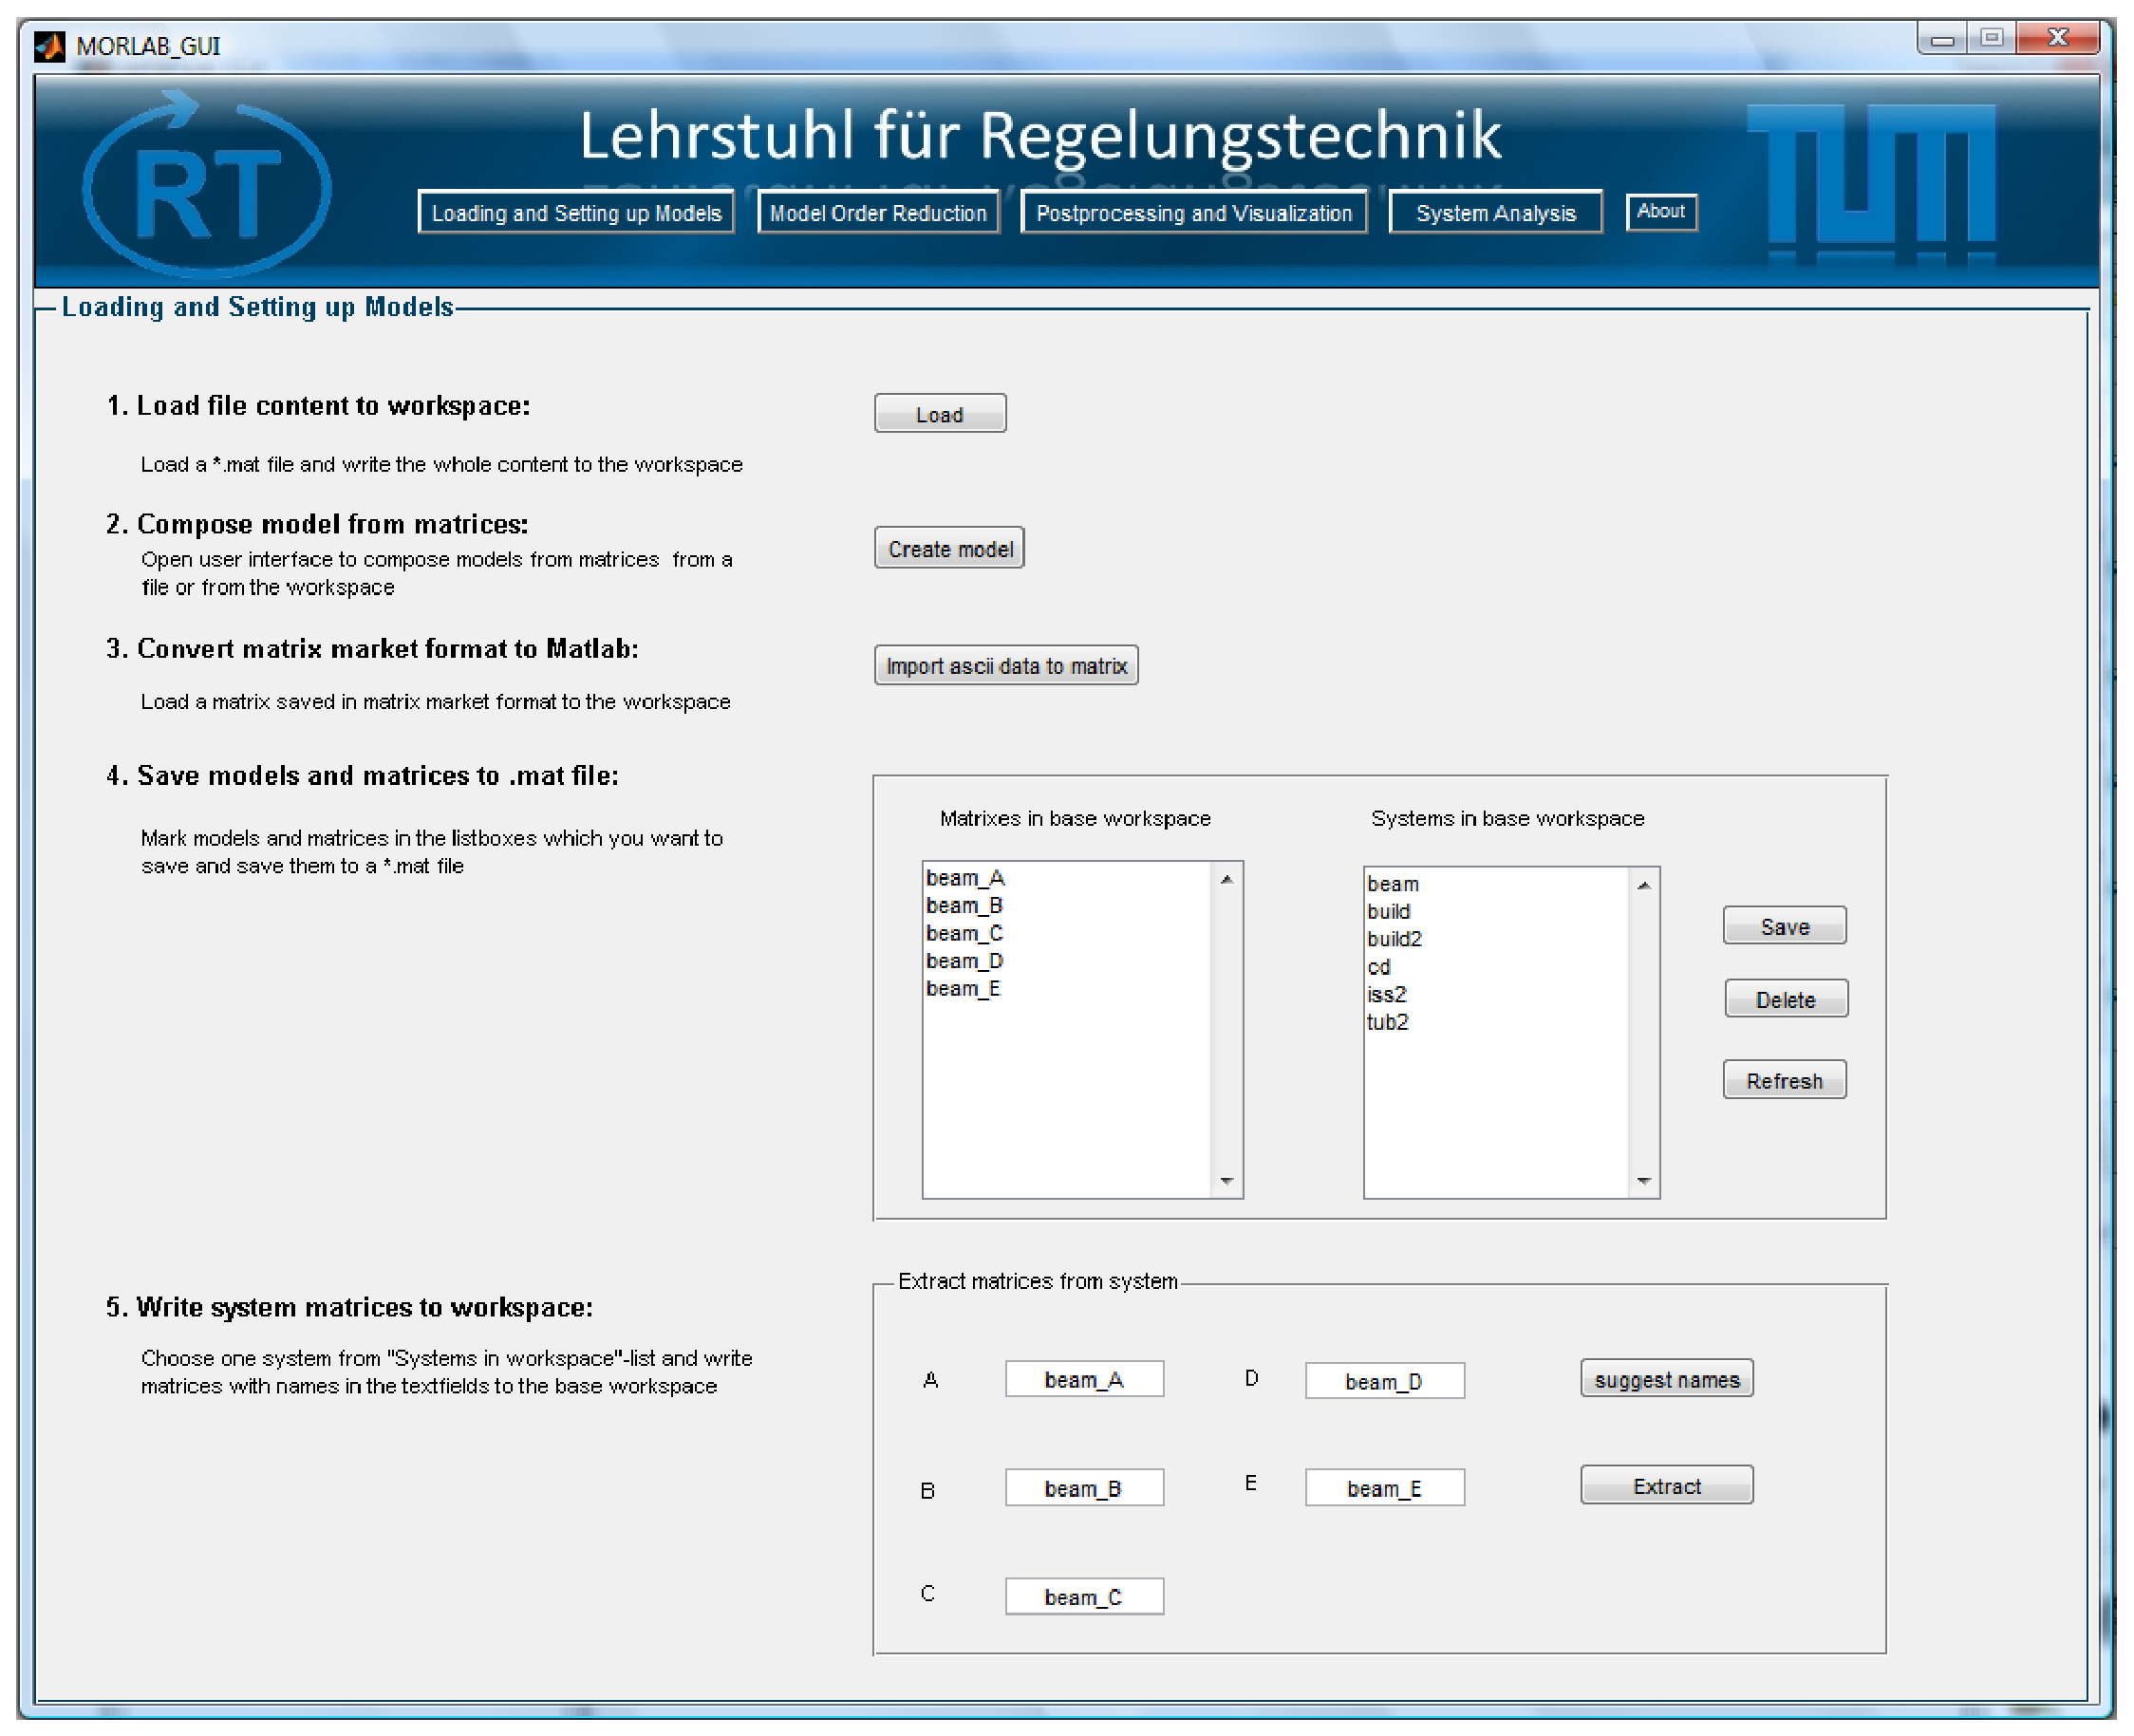
\includegraphics[width=\linewidth,height=\textheight,keepaspectratio]{Abbildungen/tab_loading}
\caption{Tab Load and Save Models}
\end{figure}
Die GUI arbeitet nicht mit dem in Matlab �blichen ss Format, sondern speichert die Matrizen A,B,C,D und E in einem Struct ab. So k�nnen zus�tzliche Informationen, wie beispielsweise Pole und Nullstellen oder Normen gemeinsam mit dem System gespeichert werden und m�ssen nur einmal berechnet werden.

\subsection{Komplette Dateien laden}
Mit 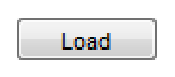
\includegraphics[height=12pt,keepaspectratio]{Abbildungen/pb_load} besteht die M�glichkeit ganze Dateien zu laden. Diese m�ssen im .mat Format vorliegen. Hierbei werden Namenskonflikte nicht �berpr�ft und vorhandene Variablen mit gleichem Namen �berschrieben.

\subsection{Matrizen importieren}
Matrizen, die im Matrix Market Format vorliegen, k�nnen mit 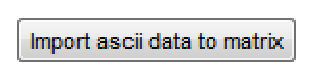
\includegraphics[height=12pt,keepaspectratio]{Abbildungen/pb_import} importiert werden.
Beispiel f�r eine Matrix im MM Format:\vspace{5mm}\\
\begin{small}
\texttt{\% Kommentarzeilen\\
\% A ist eine sparse Matrix, Gr��e 3x3 mit 5 von Null \\
\% verschiedenen Eintr�gen\\
3 3 5\\
1 1 2.0\\
1 2 6.1\\
2 1 5.0\\
2 3 -6.3\\
3 3 1.0\vspace{5mm}\\
}
\end{small}Als erstes �ffnet sich ein Dialog Fenster, in welchem die Datei, in der die Matrix gespeichert ist, auszuw�hlen ist. 
Im n�chsten Schritt muss ein Name f�r die Matrix festgelegt werden. Hier wird �berpr�ft, ob sich bereits eine Variable mit diesem Namen im Workspace befindet. Gegebenenfalls wird die M�glichkeit geboten, den Namen zu �ndern, um keine vorhandenen Variablen zu �berschreiben.
Beim Matrix Market Format ist es �blich, von symmetrischen Matrizen nur eine H�lfte zu speichern. Falls eine Dreiecksmatrix vorliegt, �ffnet sich erneut ein Fenster, in dem gew�hlt werden kann, ob die Matrix gespiegelt werden soll, oder nicht.
Nach dem erfolgreichen Ladevorgang erscheint eine Best�tigung.

%"`Create Model"'
\subsection{Systeme zusammensetzen}
Zum Erstellen von Systemen existiert eine Eingabemaske. (Abb. 2) Diese kann �ber 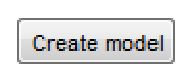
\includegraphics[height=12pt,keepaspectratio]{Abbildungen/pb_create}  aufgerufen werden. Dabei werden zwei Systemdarstellungen unterst�tzt:
\begin{align*}
\mathbf{E \dot{x}}= &\mathbf{A x} + \mathbf{B u} \hspace{20mm} 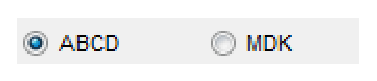
\includegraphics[height=16pt,keepaspectratio]{Abbildungen/abc} \\
\mathbf{y}=  &\mathbf{C x} + \mathbf{Du}
\end{align*}
und Systeme zweiter Ordnung:
\begin{align*}
\mathbf{M \ddot{z}} + \mathbf{D \dot{z}} +\mathbf{K z} = \mathbf{B u}& \hspace{9mm} 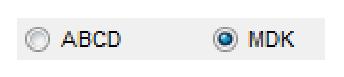
\includegraphics[height=15pt,keepaspectratio]{Abbildungen/mdk} \\
\mathbf{y}=\mathbf{C_x z} + \mathbf{C_v \dot{z}}&
\end{align*}
Systeme zweiter Ordnung werden automatisch in eine \textit{Zustandsraumdarstellung} umgewandelt.
\begin{align*}
&\overbrace{\begin{bmatrix}\mathbf{F} & \mathbf{0}\\\mathbf{0} & \mathbf{M}\end{bmatrix}}^{\mathbf{E}}
\overbrace{\begin{bmatrix}\mathbf{\dot{z}}\\ \mathbf{\ddot{z}}\end{bmatrix}}^{\mathbf{\dot{x}}} =
\overbrace{\begin{bmatrix} \mathbf{0} & \mathbf{F}\\ \mathbf{-K}&\mathbf{-D} \end{bmatrix}}^{\mathbf{A}}
\overbrace{\begin{bmatrix}\mathbf{z}\\\mathbf{\dot{z}}\end{bmatrix}}^{\mathbf{x}}+
\overbrace{\begin{bmatrix}\mathbf{0}\\\mathbf{B}\end{bmatrix}}^{\mathbf{B}}\mathbf{u}\\
&\mathbf{y} = \underbrace{\begin{bmatrix}\mathbf{C_x}&\mathbf{C_v}\end{bmatrix}}_{\mathbf{C}}
\begin{bmatrix}\mathbf{z}\\\mathbf{\dot{z}}\end{bmatrix}
\end{align*}
\begin{figure}[htb]
\noindent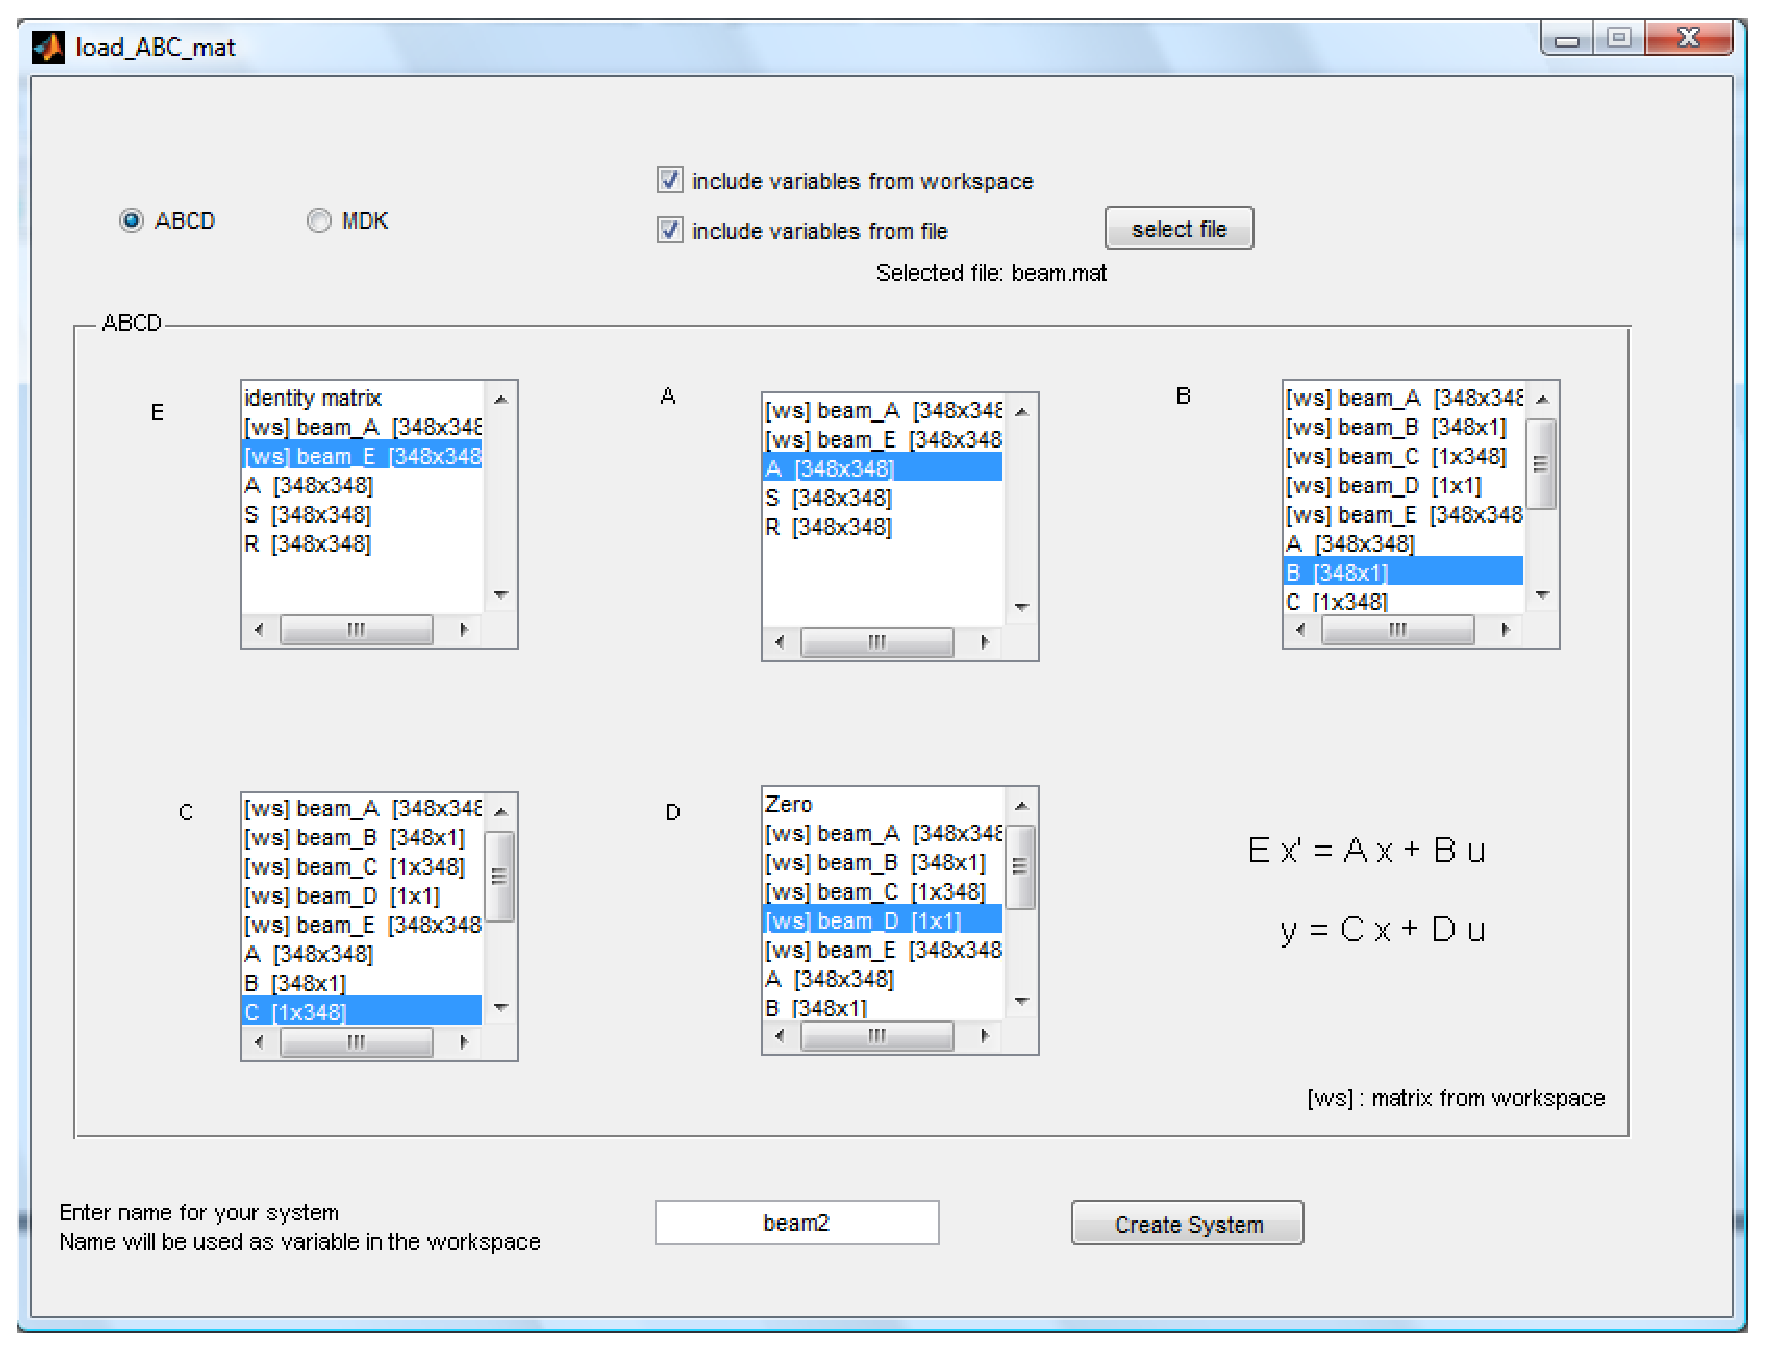
\includegraphics[width=\linewidth,keepaspectratio]{Abbildungen/tab_load_abc}%
\caption{Eingabemaske zur Erstellung von Systemen}%
\end{figure}%"`include Variables from workspace"'"`include variables from file"'"`create system"'
Die Matrizen aus denen ein System erstellt werden soll, k�nnen entweder aus dem Matlab Workspace stammen, oder in einer *.mat Datei gespeichert sein. Im ersten Fall muss das Kontrollk�stchen 
\includegraphics[height=12pt,keepaspectratio]{Abbildungen/cb_includevariablesfws}  aktiviert werden. Allen Matrizen aus dem Workspace wird ein [ws] vorangestellt.  Eine Datei kann �ber "`select file"' ausgew�hlt werden. Das Kontrollk�stchen 
\includegraphics[height=12pt,keepaspectratio]{Abbildungen/cb_includevariablesff} ist au�erdem zu aktivieren. Die Datei wird nicht komplett in den Workspace geschrieben, es besteht also nicht die Gefahr, Variablen zu �berschreiben.
Der Name, den das System im Workspace tragen soll, muss im Textfeld am unteren Rand der Eingabemaske eingetragen werden. Falls bereits eine Variable mit diesem Namen existiert, erscheint eine Warnung.
Nachdem in jedem Auswahlfeld eine Matrix ausgew�hlt wurde, kann das System �ber 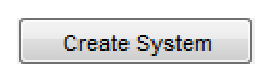
\includegraphics[height=12pt,keepaspectratio]{Abbildungen/pb_createsys} in den Workspace geschrieben werden.
Der Nutzer erh�lt eine Erfolgsmeldung und die M�glichkeit weitere Systeme zu kreieren, oder die Eingabemaske zu schlie�en.

\subsection{Systeme und Matrizen im Workspace verwalten}%"`Save"'"`Delete"'"`Refresh"'
Alle Systeme und Matrizen, die im Workspace liegen, werden auf der "`Load and Save Models"'  Seite angezeigt. 
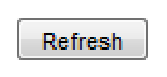
\includegraphics[height=12pt,keepaspectratio]{Abbildungen/pb_refresh}  aktualisiert die Listen. Mit 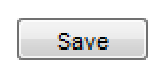
\includegraphics[height=12pt,keepaspectratio]{Abbildungen/pb_save} k�nnen alle markierten Matrizen und Systeme in einer *.mat Datei gespeichert werden, oder mit 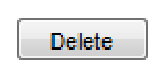
\includegraphics[height=12pt,keepaspectratio]{Abbildungen/pb_delete} aus dem  Workspace gel�scht werden.

\subsection{Matrizen aus Systemen extrahieren}%"`extract"'"`suggest names"'
Um verschiedene Systemmatrizen zu neuen Systemen zu kombinieren, k�nnen einzelne, oder mehrere Matrizen aus einem System in den Workspace geschrieben werden. Dazu muss in der "`Systems in base Workspace"' Liste ein System markiert werden. Ein automatischer Namensvorschlag kann �ber 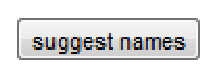
\includegraphics[height=12pt,keepaspectratio]{Abbildungen/pb_suggestnames} generiert werden. Leere Namensfelder bewirken, dass die entsprechenden Matrizen nicht in den Workspace geschrieben werden. 
Nach der Eingabe eines Matrizennamens erscheint eine Warnmeldung, falls bereits eine Variable mit dem gleichen Namen im Workspace vorliegt.
Der Vorgang wird mit 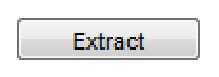
\includegraphics[height=12pt,keepaspectratio]{Abbildungen/pb_extract} gestartet. Anschlie�end erscheint eine Best�tigung.